\section{Introduction}
\label{sec:background}

About 4 pages that introduces in (sufficient) depth the key concepts
and architecture of the technology.  May use a running example to
introduce the technology.

This part and other parts of the report probably needs to refer to
figures. Figure~\ref{fig:framework} from \cite{brown:96} just
illustrates how figure can be included in the report.

\begin{figure}
  \centering
  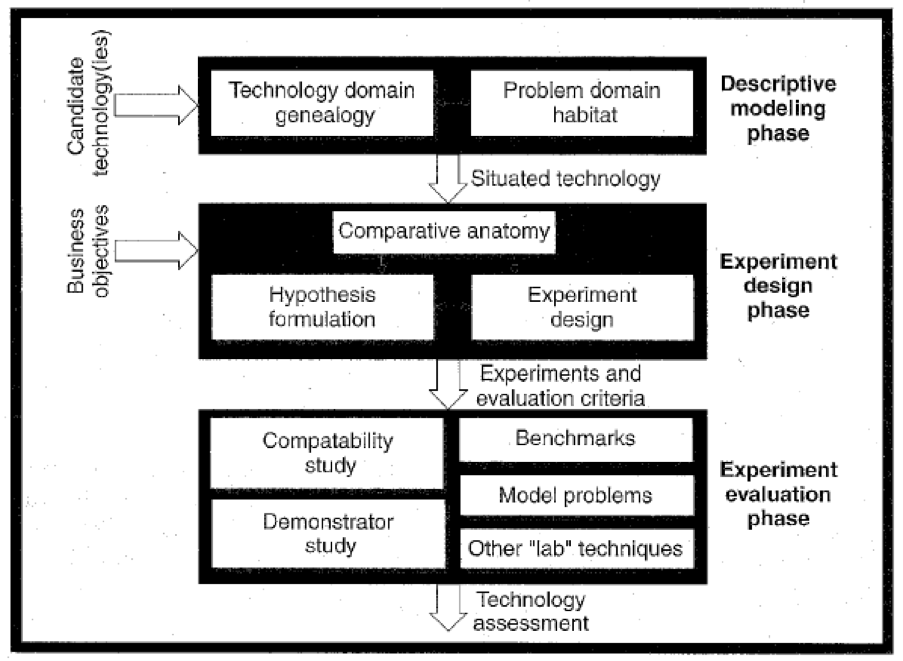
\includegraphics[scale=0.5]{figs/framework.png}
  \caption{Software technology evaluation framework.}
  \label{fig:framework}
\end{figure}


\subsection{Motivation}
we are a motivated lot ,';j

\subsection{Kotlin}

\subsubsection{What is Kotlin?}
\subsubsection{History}
\subsubsection{Functionality}
\subsubsection{Where to use Kotlin}



\subsection{Kotlin Syntax}
 -On the Syntax of Kotlin (some examples)
 



